\documentclass[12pt,a4paper]{article}
\usepackage{fontspec}
\setmainfont{Latin Modern Roman}
\setsansfont{Latin Modern Sans}
\IfFileExists{lithuanian.ldf}{\usepackage[lithuanian]{babel}}{\usepackage[provide=*]{babel}\babelprovide[main,import]{lithuanian}}
\usepackage{amsmath,amssymb,multicol,enumitem,needspace,tikz,tcolorbox}
\usepackage[left=1.6cm,right=1.6cm,top=1.5cm,bottom=1.5cm]{geometry}
\emergencystretch=2em
\setlength{\parindent}{0pt}\setlength{\parskip}{3pt}
\setlist[enumerate,1]{label=\textbf{\arabic*.},ref=\arabic*,leftmargin=*,itemsep=7pt}
\setlist[enumerate,2]{label=\alph*),leftmargin=*,itemsep=3pt}
\newcommand{\zingsnis}[1]{\tikz[baseline=(z.base)]\node[draw=black!65,fill=black!7,circle,inner sep=1pt,minimum size=5mm,font=\sffamily\bfseries\footnotesize] (z) {#1};}
% Skaičių tiesė su dviem atstumais iki ekstremumo taško.
\newcommand{\atstumai}[8]{%
\par\needspace{3.2cm}\begin{center}\begin{tikzpicture}[x=1.15cm,y=1cm,>=stealth]
\pgfmathsetmacro{\xmin}{min(#1,min(#2,#3))-0.8}
\pgfmathsetmacro{\xmax}{max(#1,max(#2,#3))+0.8}
\draw[->,black!70] (\xmin,0)--(\xmax,0) node[right] {$x$};
\draw[black!45,densely dotted] (#1,-0.15)--(#1,1.22);
\foreach \t in {#1,#2,#3} {\draw (\t,-0.08)--(\t,0.08);}
\fill[teal!70!black] (#1,0) circle (2pt) node[below=3pt,black] {$#4$};
\fill[blue!70!black] (#2,0) circle (1.8pt) node[below=3pt,black] {$#5$};
\fill[orange!85!black] (#3,0) circle (1.8pt) node[below=3pt,black] {$#6$};
\draw[<->,blue!70!black,thick] (#1,0.45)--node[above,fill=white,inner sep=1pt] {\small $#7$} (#2,0.45);
\draw[<->,orange!85!black,thick] (#1,1.00)--node[above,fill=white,inner sep=1pt] {\small $#8$} (#3,1.00);
\draw[blue!55,densely dotted] (#2,0.08)--(#2,0.45);
\draw[orange!75!black,densely dotted] (#3,0.08)--(#3,1.00);
\end{tikzpicture}\end{center}%
}
\newcommand{\svarbu}{\tikz[baseline=(zenklas.base)]\node[circle,draw=blue!50!black,line width=0.6pt,minimum size=4.5mm,inner sep=0pt,font=\sffamily\bfseries\small,text=blue!50!black] (zenklas) {!};}
\begin{document}
\begin{center}{\large\sffamily\bfseries KVADRATINIS DAUGIANARIS}\\[5pt]{\small\sffamily 5 TEMA}\\[4pt]{\Large\bfseries Daugianario reikšmių simetrija}\\[7pt]{\small Andrius Berniukevičius \quad\textbar\quad Vilniaus licėjus}\\[4pt]\rule{0.72\textwidth}{0.4pt}\end{center}
\begin{tcolorbox}[colback=black!3,colframe=black!65,boxrule=0.6pt,arc=2mm,left=2.5mm,right=2.5mm,top=1.5mm,bottom=1.5mm]
\textbf{Kaip dirbti su šia medžiaga?}

Ši medžiaga skirta aktyviam mokymuisi: naujas mintis ir faktus atrasi spręsdamas uždavinius.
\begin{enumerate}[label=\protect\zingsnis{\arabic*},leftmargin=8mm,itemsep=1pt,topsep=2pt]
\item \textbf{Pirmiausia galvok pats.} Perskaityk sąlygą, išbandyk savo idėjas pasitelkdamas pavyzdžius ir užrašyk sprendimą taip, kaip supranti. Jei užstrigai, išbandyk konkretų skaičių arba grįžk prie panašaus ankstesnio uždavinio.
\item \textbf{Tik tada pasitikrink.} Palygink savo sprendimą su pateiktuoju. Tavo būdas gali skirtis nuo pateiktojo ir vis tiek būti teisingas. Jei suklydai, išsiaiškink savo klaidą. Jei pasinaudojai pateiktu sprendimu, išnagrinėk, kodėl kiekvienas jo žingsnis teisingas. Tada užversk sprendimą ir išspręsk uždavinį iš naujo pats.
\item \textbf{Sustok prie $\star$.} Žvaigždute pažymėti uždaviniai padeda atrasti ir suprasti svarbias idėjas, kuriomis remsimės šioje ir vėlesnėse temose. Juos išsprendęs, pabandyk savais žodžiais nusakyti, ką sužinojai ir kodėl tai teisinga.
\item \textbf{Apibendrink ir pasitikrink.} Temos pabaigoje rasi svarbiausias išvadas. Pirmiausia pamėgink jas prisiminti pats, tada palygink su pateiktomis. Savikontrolės uždavinį ($\blacklozenge$) spręsk užvertęs santrauką, o po pertraukos prie jo sugrįžk.
\end{enumerate}
Siek ne vien gauti teisingą atsakymą, bet ir suprasti, \textbf{kodėl jis teisingas ir kada atrastą mintį galėsi pritaikyti}.
\end{tcolorbox}
\textbf{Temos esmė ir tikslas.} Tyrinėsi kvadratinio daugianario reikšmių simetriją ekstremumo taško atžvilgiu. Išmoksi naudotis vienodais ir skirtingais atstumais reikšmėms lyginti bei daugianariams sudaryti.

\textbf{Prieš pradėdamas:} mokėk apskaičiuoti daugianario reikšmes (1 tema), išskirti pilnąjį kvadratą (2 tema), rasti ekstremumo tašką ir ekstremumą (3–4 temos). Visur $x$ ir kiti kintamieji yra realieji skaičiai. Šioje temoje grafikų nenagrinėjame.
\begin{enumerate}
\item Duotas $P(x)=2(x-3)^2+1$.
\begin{enumerate}
\item Raskite ekstremumo tašką ir ekstremumą.
\item Apskaičiuokite ir palyginkite $P(2)$ ir $P(4)$; $P(1)$ ir $P(5)$; $P(0)$ ir $P(6)$.
\item Ar kiekvienos poros skaičiai yra vienodai nutolę nuo skaičiaus $3$? Paaiškinkite.
\item Raskite $P(3-t)$ ir $P(3+t)$. Ar jie lygūs visiems realiesiems $t$? Paaiškinkite.
\end{enumerate}
\item Kvadratinio daugianario $P(x)=2(x-2)^2+1$ ekstremumo taškas yra $h=2$. Skaičių tiesėje pažymėti trys skaičiai.
\begin{center}\begin{tikzpicture}[x=1.05cm,>=stealth]
\draw[->,black!70] (-1.6,0)--(5.6,0) node[right] {$x$};
\foreach \x in {-1,0,1,2,3,4,5}{\draw (\x,-0.07)--(\x,0.07);\node[below=3pt] at (\x,0) {$\x$};}
\fill[blue!70!black] (0,0) circle (2pt);\fill[teal!70!black] (2,0) circle (2.4pt);\fill[orange!85!black] (4,0) circle (2pt);
\node[above=5pt,teal!70!black] at (2,0) {$h$};
\end{tikzpicture}\end{center}
\begin{enumerate}
\item Kokiais atstumais nuo $h$ yra skaičiai $0$ ir $4$? Ką pastebite?
\item Apskaičiuokite ir palyginkite $P(0)$ ir $P(4)$. Paaiškinkite, kaip šių reikšmių lygybė susijusi su atstumais nuo $h$.
\item Remdamiesi brėžiniu, raskite kitą skaičių, su kuriuo daugianario reikšmė tokia pati kaip $P(1)$. Patikrinkite skaičiuodami.
\end{enumerate}
\item $\star$ Kvadratinio daugianario $P(x)=a(x-h)^2+k$ ekstremumo taškas yra $h$, kur $a\ne0$. Skaičių tiesėje parodytas atvejis $t>0$.
\begin{center}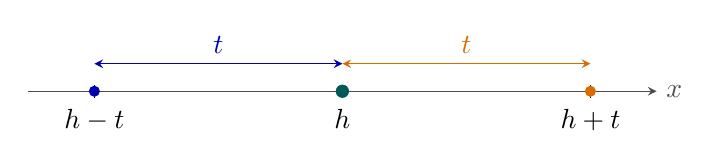
\begin{tikzpicture}[x=1.05cm,>=stealth]
\draw[->,black!70] (-3.8,0)--(3.8,0) node[right] {$x$};
\foreach \z in {-3,0,3}{\draw (\z,-0.08)--(\z,0.08);}
\fill[blue!70!black] (-3,0) circle (2pt) node[below=3pt,black] {$h-t$};
\fill[teal!70!black] (0,0) circle (2.4pt) node[below=3pt,black] {$h$};
\fill[orange!85!black] (3,0) circle (2pt) node[below=3pt,black] {$h+t$};
\draw[<->,blue!70!black] (-3,0.35)--node[above] {$t$} (0,0.35);
\draw[<->,orange!85!black] (0,0.35)--node[above] {$t$} (3,0.35);
\end{tikzpicture}\end{center}
\begin{enumerate}
\item Įrodykite, kad kiekvienam realiajam $t$ galioja $P(h-t)=P(h+t)$.
\item Paaiškinkite šios lygybės prasmę, kai $t>0$. Kokiu atstumu nuo $h$ yra skaičiai $h-t$ ir $h+t$?
\item Ar lygybė galioja, kai $t=0$? O kai $t<0$? Paaiškinkite, kas tada nutinka skaičiams $h-t$ ir $h+t$.
\end{enumerate}
\par\medskip
\textbf{Sustokite ir apibendrinkite.} Kodėl skaičiai $h-t$ ir $h+t$ duoda tą pačią daugianario reikšmę? Kaip rasti skaičiui $u$ simetrišką skaičių?
\item Daugianario ekstremumo taškas yra $h$, o $u\ne h$. Raskite kitą skaičių $v\ne u$, su kuriuo $P(v)=P(u)$, ir apskaičiuokite $P(v)$.
\begin{enumerate}
\item $h=3$, $u=1$, $P(1)=7$;
\item $h=-2$, $u=1$, $P(1)=-5$;
\item $h=\frac{1}{2}$, $u=-1$, $P(-1)=4$;
\item $h=-3$, $u=-5$, $P(-5)=0$.
\end{enumerate}
\item Skaičių tiesėje pažymėti skirtingi skaičiai $2$ ir $8$. Žinoma, kad kvadratiniam daugianariui $P$ galioja $P(2)=P(8)$.
\begin{center}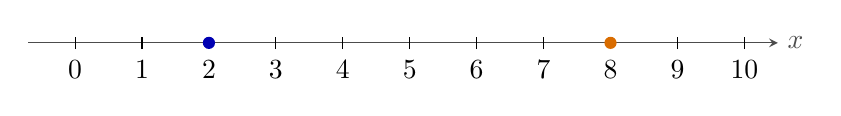
\begin{tikzpicture}[x=0.85cm,>=stealth]
\draw[->,black!70] (-0.7,0)--(10.5,0) node[right] {$x$};
\foreach \x in {0,...,10}{\draw (\x,-0.08)--(\x,0.08);\node[below=3pt] at (\x,0) {$\x$};}
\fill[blue!70!black] (2,0) circle (2.2pt);\fill[orange!85!black] (8,0) circle (2.2pt);
\end{tikzpicture}\end{center}
\begin{enumerate}
\item Kuris brėžinyje pažymėtas skaičius yra tiksliai per vidurį tarp $2$ ir $8$? Kokiais atstumais nuo jo yra abu skaičiai?
\item Remdamiesi anksčiau nagrinėta simetrija, iškelkite hipotezę: kur turėtų būti daugianario ekstremumo taškas?
\item Jeigu skirtingiems skaičiams $u$ ir $v$ galioja $P(u)=P(v)$, kokia formule galima apskaičiuoti ekstremumo tašką $h$? Paaiškinkite, kodėl brėžinio nepakanka šiai formulei įrodyti.
\end{enumerate}
\textit{Kitame uždavinyje šią hipotezę įrodysime.}
\item\label{vidurio-irodymas} $\star$ Duotas kvadratinis daugianaris $P(x)=a(x-h)^2+k$, kur $a\ne0$, o $h$ yra ekstremumo taškas. Žinoma, kad $P(u)=P(v)$ ir $u\ne v$. Įrodysime, kad $h=\frac{u+v}{2}$.
\begin{enumerate}
\item Į daugianarį vietoj $x$ įrašykite $u$ ir $v$. Užrašykite $P(u)$ ir $P(v)$.
\item Pasinaudodami lygybe $P(u)=P(v)$, parodykite, kad $(u-h)^2=(v-h)^2$.
\item Pasinaudokite savybe: jei dviejų realiųjų skaičių kvadratai lygūs, tai tie skaičiai yra lygūs arba priešingi. Pavyzdžiui, jei $z^2=9$, tai $z=3$ arba $z=-3$. Kokias dvi lygybes gaunate iš b) dalies?
\item Kurią iš gautų lygybių atmetame, nes $u\ne v$? Iš kitos lygybės išveskite formulę $h=\frac{u+v}{2}$.
\item Kodėl šios išvados negalima daryti, jei sąlygos $u\ne v$ atsisakome? Pateikite pavyzdį.
\end{enumerate}
\par\medskip
\textbf{Sustokite ir apibendrinkite.} Kada iš lygybės $P(u)=P(v)$ galima rasti ekstremumo tašką? Kodėl būtina sąlyga $u\ne v$?
\item Nustatykite ekstremumo tašką:
\begin{enumerate}
\item $P(1)=P(7)$; \item $P(-4)=P(2)$; \item $P(-3)=P(5)$; \item $P(0)=P(-6)$.
\end{enumerate}
Ar iš pateiktų duomenų galima nustatyti, ar bent vieno daugianario ekstremumas yra minimumas, ar maksimumas? Paaiškinkite.
\item Išnagrinėkite teiginius, nurodykite, kurie iš jų teisingi, ir pagrįskite atsakymus.
\begin{enumerate}
\item Jeigu $P(2)=P(6)$, tai ekstremumo taškas yra $4$.
\item Jeigu $P(3)=P(3)$, tai ekstremumo taškas yra $3$.
\item Jeigu $h=2$ ir $P(0)=5$, tai $P(4)=5$.
\item Jeigu $P(1)=P(7)$, tai būtinai $P(2)=P(5)$.
\end{enumerate}
\item $\star$ Raskite visas kintamojo reikšmes, kurioms kvadratinio daugianario reikšmės yra lygios.
\begin{enumerate}
\item Kvadratinio daugianario $P$ ekstremumo taškas yra $h=3$. Raskite dvi skirtingas $x$ reikšmes, su kuriomis daugianario reikšmė lygi $P(1)$. Paaiškinkite, kodėl abi rastos reikšmės tinka.
\begin{center}\begin{tikzpicture}[x=0.95cm,>=stealth]
\draw[->,black!70] (-0.6,0)--(6.7,0) node[right] {$x$};
\foreach \z in {0,...,6}{\draw (\z,-0.08)--(\z,0.08);\node[below=3pt] at (\z,0) {$\z$};}
\fill[blue!70!black] (1,0) circle (2pt);\fill[teal!70!black] (3,0) circle (2.4pt);
\node[above=5pt,teal!70!black] at (3,0) {$h$};
\end{tikzpicture}\end{center}
\item Tarkime, kad ieškoma antroji $x$ reikšmė nėra $1$. Remdamiesi \ref{vidurio-irodymas} uždavinio išvada, ją raskite. Paaiškinkite, kodėl, be a) dalyje rastųjų, kitų tinkamų reikšmių nėra.
\item Tegul kvadratinio daugianario $P$ ekstremumo taškas yra $h$, o $u$ – pasirinktas realusis skaičius. Remdamiesi ankstesnėmis dalimis ir \ref{vidurio-irodymas} uždaviniu, raskite visas $v$ reikšmes, su kuriomis daugianario reikšmė $P(v)$ lygi $P(u)$. Patikrinkite, ar jos tinka.
\item Kas nutinka, kai $u=h$? Kiek skirtingų $v$ reikšmių tada tinka? Kiek jų tinka, kai $u\ne h$?
\end{enumerate}
\par\medskip
\textbf{Sustokite ir apibendrinkite.} Kiek skirtingų $x$ reikšmių gali duoti tą pačią kvadratinio daugianario reikšmę? Kas pasikeičia, jei žinoma reikšmė yra ekstremumas?
\item Palyginkite kiekvienoje dalyje nurodytas reikšmes, jų neapskaičiuodami. Jei reikšmės lygios, paaiškinkite kodėl.
\begin{enumerate}
\item $P(x)=2(x-3)^2+1$: palyginkite $P(1)$ ir $P(6)$.
\item $Q(x)=-3(x-2)^2+5$: palyginkite $Q(1)$ ir $Q(5)$.
\item $R(x)=4(x+1)^2-3$: palyginkite $R(-4)$ ir $R(2)$.
\item $S(x)=-(x+2)^2+7$: palyginkite $S(-1)$ ir $S(-4)$.
\end{enumerate}
\item Skaičių tiesėje parodytas kvadratinio daugianario $P(x)=a(x-1)^2+k$ ekstremumo taškas $h=1$ ir skaičiai $-1$ bei $4$.
\begin{center}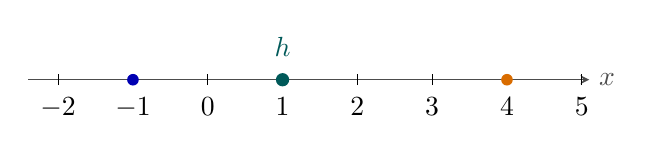
\begin{tikzpicture}[x=0.95cm,>=stealth]
\draw[->,black!70] (-2.4,0)--(5.1,0) node[right] {$x$};
\foreach \x in {-2,-1,0,1,2,3,4,5}{\draw (\x,-0.07)--(\x,0.07);\node[below=3pt] at (\x,0) {$\x$};}
\fill[blue!70!black] (-1,0) circle (2.1pt);\fill[teal!70!black] (1,0) circle (2.4pt);\fill[orange!85!black] (4,0) circle (2.1pt);
\node[above=5pt,teal!70!black] at (1,0) {$h$};
\end{tikzpicture}\end{center}
\begin{enumerate}
\item Kokiu atstumu nuo $h$ yra kiekvienas iš skaičių $-1$ ir $4$? Kuris skaičius arčiau $h$?
\item Palyginkite $P(-1)$ ir $P(4)$, jeigu $a>0$. Pasinaudokite atstumais ir duotu daugianario pavidalu.
\item Palyginkite $P(-1)$ ir $P(4)$, jeigu $a<0$. Paaiškinkite, kas pasikeitė.
\item Ar galima šias reikšmes palyginti, jei $a$ ženklas nežinomas? Pagrįskite dviejų daugianarių pavyzdžiais.
\end{enumerate}
\item \textbf{Skaičiaus modulis.} Skaičiaus $z$ moduliu vadinamas atstumas skaičių tiesėje nuo taško, kurio koordinatė $z$, iki taško $0$. Modulis žymimas $|z|$. Pavyzdžiui, $|3|=3$, $|-3|=3$, $|0|=0$. Kitaip tariant,
\[
|z|=\begin{cases}z,&\text{kai }z\ge0,\\-z,&\text{kai }z<0.\end{cases}
\]
\begin{center}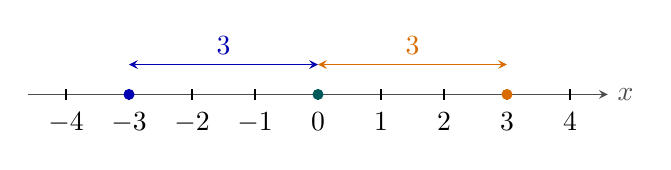
\begin{tikzpicture}[x=0.8cm,>=stealth]
\draw[->,black!70] (-4.6,0)--(4.6,0) node[right] {$x$};
\foreach \z in {-4,...,4}{\draw (\z,-0.07)--(\z,0.07);\node[below=3pt] at (\z,0) {$\z$};}
\fill[blue!70!black] (-3,0) circle (2pt);\fill[teal!70!black] (0,0) circle (2pt);\fill[orange!85!black] (3,0) circle (2pt);
\draw[<->,blue!70!black] (-3,0.38)--node[above] {$3$} (0,0.38);
\draw[<->,orange!85!black] (0,0.38)--node[above] {$3$} (3,0.38);
\end{tikzpicture}\end{center}
\begin{enumerate}
\item Apskaičiuokite $|-5|$, $|2|$, $|0|$, $|-\frac{3}{2}|$.
\item Raskite visus skaičius $z$, kuriems $|z|=4$. Kiek sprendinių turi lygtis $|z|=0$? O lygtis $|z|=-1$? Paaiškinkite.
\item Paaiškinkite, kodėl kiekvienam realiajam $z$ galioja $|z|^2=z^2$. Panaudokite modulio apibrėžime pateiktus du atvejus.
\end{enumerate}
\item $\star$ \textbf{Modulis ir atstumas tarp dviejų taškų.} Atstumas skaičių tiesėje tarp taškų, kurių koordinatės $u$ ir $h$, yra $|u-h|$. Jei $u\ge h$, tai atstumas yra $u-h$; jei $u<h$, tai atstumas yra $h-u$. Abu atvejus užrašo reiškinys $|u-h|$.
\begin{center}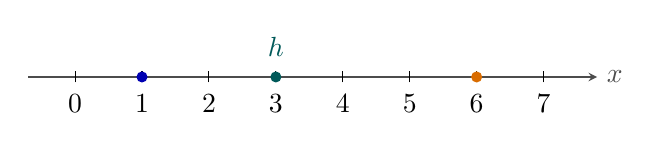
\begin{tikzpicture}[x=0.85cm,>=stealth]
\draw[->,black!70] (-0.7,0)--(7.8,0) node[right] {$x$};
\foreach \z in {0,...,7}{\draw (\z,-0.07)--(\z,0.07);\node[below=3pt] at (\z,0) {$\z$};}
\fill[blue!70!black] (1,0) circle (2pt);\fill[teal!70!black] (3,0) circle (2pt);\fill[orange!85!black] (6,0) circle (2pt);
\node[above=4pt,teal!70!black] at (3,0) {$h$};
\end{tikzpicture}\end{center}
\begin{enumerate}
\item Kai $h=3$, skaičių tiesėje raskite atstumus nuo $1$ ir nuo $6$ iki $h$. Patikrinkite juos apskaičiuodami $|1-3|$ ir $|6-3|$.
\item Kai $h=-2$, raskite atstumus nuo $-5$ ir nuo $1$ iki $h$. Ką pastebite?
\item Paaiškinkite, kodėl visiems realiesiems $u$ ir $h$ galioja $|u-h|^2=(u-h)^2$.
\end{enumerate}
\item $\star$ Kvadratinis daugianaris užrašytas pavidalu $P(x)=a(x-h)^2+k$, kur $a\ne0$. Tarkime, kad skaičius $u$ yra arčiau ekstremumo taško $h$ negu skaičius $v$.
\begin{enumerate}
\item Atstumus užrašykite moduliais ir paaiškinkite, kodėl $(u-h)^2<(v-h)^2$.
\item Įrodykite, kad kai $a>0$, tai $P(u)<P(v)$, o kai $a<0$, tai $P(u)>P(v)$.
\item Suformuluokite taisyklę žodžiais. Kas būtų, jei $u$ ir $v$ nuo $h$ būtų nutolę vienodai?
\end{enumerate}
\par\medskip
\textbf{Sustokite ir apibendrinkite.} Kaip atstumai iki ekstremumo taško ir $a$ ženklas padeda palyginti daugianario reikšmes?
\item Kiekvienoje dalyje pateiktas kvadratinis daugianaris $P(x)=ax^2+bx+c$, tačiau jo koeficientai nežinomi. Palyginkite nurodytas daugianario reikšmes, prieš tai radę ekstremumo tašką ir palyginę atstumus nuo jo. Pačių reikšmių apskaičiuoti nereikia.
\begin{enumerate}
\item $a<0$, $P(2)=P(8)$: palyginkite $P(7)$ ir $P(9)$.
\item $a>0$, $P(1)=P(5)$: palyginkite $P(3)$ ir $P(4)$.
\item $a>0$, $P(-4)=P(2)$: palyginkite $P(-3)$ ir $P(2)$.
\item $a<0$, $P(-2)=P(4)$: palyginkite $P(-3)$ ir $P(3)$.
\item $a>0$, $P(0)=P(5)$: palyginkite $P(1)$ ir $P(4)$.
\item $a<0$, $P(-5)=P(1)$: palyginkite $P(-2)$ ir $P(-3)$.
\end{enumerate}
\item Žinoma, kad $P$ yra kvadratinis daugianaris ir $P(2)=P(8)$, tačiau vyriausiojo koeficiento ženklas nenurodytas.
\begin{enumerate}
\item Ar galima nustatyti, kuri reikšmė didesnė: $P(7)$ ar $P(9)$? Atsakymą pagrįskite dviejų daugianarių pavyzdžiais.
\item Ar galima palyginti $P(3)$ ir $P(7)$? Paaiškinkite.
\end{enumerate}
\item Palyginkite nurodytas reikšmes, jų neapskaičiuodami. Ekstremumo tašką raskite pasirinktu būdu: išskirkite pilnąjį kvadratą arba pritaikykite formulę.
\begin{enumerate}
\item $P(x)=x^2-6x+5$: $P(1)$ ir $P(6)$.
\item $Q(x)=-x^2-4x+1$: $Q(-5)$ ir $Q(0)$.
\item $R(x)=2x^2-4x+3$: $R(-1)$ ir $R(3)$.
\end{enumerate}
\item Kvadratinio daugianario $P(x)=ax^2+bx+c$ reikšmės tenkina $P(1)=P(5)$, o $a=2$ ir $P(0)=1$.
\begin{enumerate}
\item Raskite ekstremumo tašką.
\item Raskite $b$ ir $c$, užrašykite daugianarį.
\item Išskirkite pilnąjį kvadratą, raskite ekstremumą ir patikrinkite $P(1)=P(5)$.
\end{enumerate}
\item Daugianario $P$ ekstremumo taškas yra $x=2$, $P(0)=5$ ir $P(1)=2$.
\begin{enumerate}
\item Be papildomų skaičiavimų raskite $P(4)$ ir $P(3)$.
\item Sudarykite $P(x)$, išskirkite pilnąjį kvadratą ir nustatykite ekstremumą.
\item Patikrinkite gautas reikšmes įrašydami.
\end{enumerate}
\item Nustatykite, ar egzistuoja kvadratinis daugianaris, tenkinantis visas sąlygas. Jei taip, raskite visus tokius daugianarius; jei ne, pagrįskite.
\begin{enumerate}
\item Ekstremumo taškas $h=2$, $P(1)=3$, $P(3)=4$.
\item Ekstremumo taškas $h=-1$, $P(-2)=P(0)=5$.
\item $P(0)=P(4)=1$, o minimumas yra $-3$.
\item $P(0)=P(4)=1$, o maksimumas yra $3$.
\end{enumerate}
\par\bigskip
\noindent\textbf{Papildomi uždaviniai. Jungiame 1–5 temų idėjas}\par
Šie uždaviniai skirti ankstesnių temų žinioms pakartoti ir sujungti. Juos galite spręsti pasirinktinai.
\item Kvadratinis daugianaris $P(x)=ax^2+bx+c$ tenkina sąlygas $P(1)=P(5)$ ir $P(0)=2$. Ar šių duomenų pakanka, kad būtų galima nustatyti tik vieną daugianarį? Raskite visus sąlygas tenkinančius daugianarius ir patikrinkite, ar jie tinka.
\item Raskite kvadratinį daugianarį $P(x)=ax^2+bx+c$, jeigu $P(-1)=P(5)$, $a=2$ ir $P(0)=3$.
\item Daugianaris $P$ tenkina $P(-2)=P(4)$, $P(0)=3$ ir $P(3)=9$. Raskite $P(x)$, jo ekstremumo tašką ir ekstremumą.
\item Kvadratinis daugianaris $P$ tenkina $P(0)=P(4)$, jo minimumas yra $-2$, o diskriminantas $D=16$. Raskite $P(x)$ ir reikšmes $P(0)$, $P(4)$.
\item Raskite kvadratinį daugianarį $P$, jeigu $P(-3)=P(1)$, $D=0$ ir $P(0)=2$. Nustatykite ekstremumą.
\item Raskite visus kvadratinius daugianarius $P(x)=ax^2+bx+c$, jeigu $P(0)=P(4)=3$, $a>0$, $b<0$, $c>0$ ir $D<0$. Paaiškinkite, ar tokių daugianarių yra.
\item Ar egzistuoja kvadratinis daugianaris $P(x)=ax^2+bx+c$, kuriam $P(-1)=P(3)$, $a>0$ ir $b>0$? Jei taip, pateikite pavyzdį; jei ne, pagrįskite.
\item Kvadratinis daugianaris $P(x)=ax^2+bx+c$ tenkina $P(-2)=P(2)$, $a<0$, $c=4$ ir $D=16$. Raskite $P(x)$ bei jo ekstremumą.
\item Kvadratinis daugianaris $P(x)=ax^2+bx+c$ tenkina $P(-2)=P(4)$, $P(1)=-3$, $P(0)=-1$, taip pat $a>0$, $b<0$, $c<0$. Nustatykite, ar toks daugianaris egzistuoja. Jei taip, raskite jį ir apskaičiuokite $D$.
\item Raskite visus kvadratinius daugianarius $P(x)=ax^2+bx+c$, jeigu $P(-1)=P(3)$, $P(0)=2$, $a>0$, $c>0$ ir $D>0$. Pateikite vieną konkretų pavyzdį.
\item Ar egzistuoja kvadratinis daugianaris $P$, kuriam $P(-2)=P(4)$, maksimumas yra $3$, o $D=0$? Paaiškinkite remdamiesi ekstremumo ir diskriminanto ryšiu.
\end{enumerate}
\newpage
\begin{center}{\Large\bfseries Ką atradome?}\end{center}
Prieš skaitydami pabandykite iš atminties įvardyti svarbiausias temos išvadas. Tada palyginkite savo mintis su šia teorijos santrauka ir grįžkite prie vietų, kurios kelia klausimų.
\begin{tcolorbox}[colback=blue!3,colframe=blue!40!black,boxrule=0.5pt,arc=1mm,colbacktitle=blue!8,coltitle=black,title={\svarbu\quad\bfseries Svarbiausios temos išvados}]
\textbf{1. Reikšmių simetrija.} Jei $P(x)=a(x-h)^2+k$, $a\ne0$, tai visiems realiesiems $t$ galioja $P(h-t)=P(h+t)$. Skaičiui $u$ simetriškas skaičius yra $2h-u$.

\textbf{2. Ekstremumo taškas iš dviejų reikšmių.} Jei $P(u)=P(v)$ ir $u\ne v$, tai $h=\frac{u+v}{2}$. Sąlyga, kad $u$ ir $v$ skirtingi, yra būtina: lygybė $P(u)=P(u)$ neleidžia nustatyti $h$.

\textbf{3. Visos vienodos reikšmės.} Lygybė $P(v)=P(u)$ galioja tik kai $v=u$ arba $v=2h-u$. Kai $u=h$, šie skaičiai sutampa; kai $u\ne h$, jie skirtingi.

\textbf{4. Modulis ir atstumas.} Atstumas skaičių tiesėje nuo taško $u$ iki taško $h$ lygus $|u-h|$. Jis visada neneigiamas, o $|u-h|^2=(u-h)^2$.

\textbf{5. Reikšmių palyginimas.} Jei $|u-h|<|v-h|$, tai kai $a>0$ yra $P(u)<P(v)$, o kai $a<0$ – $P(u)>P(v)$. Jei atstumai vienodi, reikšmės lygios. Kai atstumai skirtingi, o $a$ ženklas nežinomas, palyginimas priklauso nuo jo.

\textbf{6. Sudarymas.} Pasinaudoję dviem skirtingais skaičiais, kuriuos atitinka tos pačios reikšmės, raskite $h$; tada iš kitų sąlygų nustatykite koeficientus, patikrinkite $a\ne0$ ir visas duotas sąlygas.
\end{tcolorbox}
\textbf{Ką verta užsirašyti į teorijos santrauką?} Pasirinkite svarbią išvadą ir užsirašykite faktą, jo sąlygas, kodėl jis teisingas, ir vieną savo pavyzdį. Išvadų taikymą pasitikrinkite toliau pateiktu $\blacklozenge$ pažymėtu uždaviniu.
\newpage
\begin{center}{\Large\bfseries Savikontrolė}\end{center}
Pirmiausia užverskite teorijos santrauką ir savarankiškai išspręskite uždavinį. Pasitikrinkite atsakymus, o jei kuri nors dalis kėlė sunkumų, grįžkite prie atitinkamos išvados ir pabandykite dar kartą. Kitą dieną arba prieš pradėdami kitą temą dar kartą išspręskite šį uždavinį nesinaudodami santrauka.
\begin{enumerate}[resume]
\item $\blacklozenge$ Atlikite užduotis ir pagrįskite atsakymus.
\begin{enumerate}
\item Kvadratiniam daugianariui $P$ galioja $P(-2)=P(6)$ ir $a<0$. Raskite ekstremumo tašką ir, neskaičiuodami reikšmių, palyginkite $P(1)$ ir $P(5)$.
\item Ekstremumo taškas yra $h=2$, o $P(0)=7$. Raskite visas $x$ reikšmes, su kuriomis $P(x)=7$.
\item Raskite kvadratinį daugianarį $Q$, jeigu $Q(0)=Q(4)=3$, o jo minimumas lygus $-1$. Patikrinkite sąlygas.
\item Žinoma, kad $P(1)=P(7)$ ir $P(2)=5$. Raskite dar vieną $x$ reikšmę, su kuria $P(x)=5$, ir paaiškinkite, kodėl kitų nėra.
\end{enumerate}
\end{enumerate}
\newpage\begin{center}{\Large\bfseries Atsakymai ir sprendimai}\end{center}
\begin{enumerate}
\item \textbf{a)} $x_{\min}=3$, $P_{\min}=1$.

\textbf{b)} $P(2)=P(4)=3$; $P(1)=P(5)=9$; $P(0)=P(6)=19$.

\needspace{5cm}\textbf{c)} Kiekvienos poros skaičiai yra skirtingose skaičiaus $3$ pusėse ir vienodai nuo jo nutolę.
\atstumai{3}{1}{5}{h=3}{1}{5}{2}{2}

\textbf{d)} $P(3-t)=2(-t)^2+1=2t^2+1$, $P(3+t)=2t^2+1$. Jie lygūs visiems $t$, nes $(-t)^2=t^2$.
\item \textbf{a)} Abu skaičiai nuo $h=2$ nutolę per $2$ vienetus: $0$ yra kairėje, o $4$ – dešinėje.

\textbf{b)} $P(0)=2(0-2)^2+1=9$, $P(4)=2(4-2)^2+1=9$. Atstumai vienodi. Skaičiai $-2$ ir $2$ yra priešingi, todėl jų kvadratai lygūs.

\textbf{c)} Skaičius $1$ nuo $2$ nutolęs per $1$, todėl simetriškas skaičius kitoje $2$ pusėje yra $3$. Patikra: $P(1)=2(-1)^2+1=3$ ir $P(3)=2\cdot1^2+1=3$.
\item \textbf{a)} $P(h-t)=a(-t)^2+k=at^2+k$, o $P(h+t)=at^2+k$, todėl reikšmės lygios.

\needspace{5cm}\textbf{b)} Jei $t>0$, skaičiai $h-t$ ir $h+t$ yra skirtingose $h$ pusėse ir abu nutolę nuo jo atstumu $t$; jų duodamos reikšmės lygios.
\textit{Brėžinys vaizduoja atvejį $t>0$.}
\atstumai{0}{-3}{3}{h}{h-t}{h+t}{t}{t}

\textbf{c)} Kai $t=0$, abu skaičiai $h-t$ ir $h+t$ lygūs $h$. Kai $t<0$, jie tik susikeičia vietomis; įrodymas su $(-t)^2=t^2$ vis tiek galioja.
\item Kita reikšmė yra $v=2h-u$.

\needspace{5cm}\textbf{a)} $v=5$, $P(5)=7$.
\atstumai{3}{1}{5}{h=3}{u=1}{v=5}{2}{2}

\textbf{b)} $v=-5$, $P(-5)=-5$.

\textbf{c)} $v=2$, $P(2)=4$.

\textbf{d)} $v=-1$, $P(-1)=0$.
\item \textbf{a)} Viduryje yra $5$; nuo jo iki $2$ ir iki $8$ yra po $3$ vienetus.

\textbf{b)} Galime numanyti, kad ekstremumo taškas yra $h=5$: tada $2$ ir $8$ yra simetriški jo atžvilgiu. Tačiau tai dar reikia įrodyti – iki šiol žinome, kad vienodai nutolusiems skaičiams reikšmės lygios, bet turime pagrįsti ir atvirkštinį teiginį.

\textbf{c)} Hipotezė: $h=\frac{u+v}{2}$. Šis brėžinys vaizduoja tik vieną atvejį, todėl vien jo nepakanka teiginiui apie visus kvadratinius daugianarius ir visus skirtingus $u$ bei $v$ įrodyti. Tai įrodoma kitame uždavinyje.
\item \textbf{a)} Įrašę $u$ ir $v$ gauname $P(u)=a(u-h)^2+k$ ir $P(v)=a(v-h)^2+k$.

\textbf{b)} Įrašę $u$ ir $v$ į $P(u)=P(v)$ gauname $a(u-h)^2+k=a(v-h)^2+k$. Iš abiejų lygybės pusių atėmę po $k$ ir padaliję iš nenulinio $a$, gauname $(u-h)^2=(v-h)^2$.

\textbf{c)} Kadangi $(u-h)^2=(v-h)^2$, tai skaičiai $u-h$ ir $v-h$ yra lygūs arba priešingi. Taigi galimi du atvejai:
\[
u-h=v-h \quad\text{arba}\quad u-h=-(v-h).
\]
Šią savybę galima pagrįsti ir taip: jeigu $p^2=q^2$, tai $(p-q)(p+q)=0$, todėl $p=q$ arba $p=-q$.

\textbf{d)} Iš pirmosios lygybės $u-h=v-h$ gautume $u=v$, o tai prieštarauja sąlygai. Todėl turi galioti antroji lygybė. Ji suderinama su $u\ne v$: pavyzdžiui, $h=3$, $u=1$, $v=5$ – tuomet $u-h=-2$ ir $v-h=2$. Iš antrosios lygybės gauname:
\[
u-h=-v+h,\qquad u+v=2h,\qquad h=\frac{u+v}{2}.
\]
\textbf{e)} Kai $u=v$, pirmoji lygybė $u-h=v-h$ galioja bet kuriam $h$, todėl iš jos negalime nustatyti ekstremumo taško. Pavyzdžiui, $P(x)=x^2$, $u=v=3$: lygybė $P(3)=P(3)$ galioja, tačiau $h=0\ne3=\frac{3+3}{2}$.
\item \textbf{a)} $h=4$. \textbf{b)} $h=-1$. \textbf{c)} $h=1$. \textbf{d)} $h=-3$. Nė vienu atveju negalima nustatyti, ar ekstremumas yra minimumas, ar maksimumas, nes nenurodytas $a$ ženklas. Pavyzdžiui, daugianariai $(x-4)^2$ ir $-(x-4)^2$ abu tenkina a) sąlygą, tačiau pirmojo ekstremumas yra minimumas, o antrojo – maksimumas.
\item \textbf{a)} Teisinga: $2\ne6$, tad $h=\frac{2+6}{2}=4$.

\textbf{b)} Neteisinga: lygybė $P(3)=P(3)$ galioja bet kuriam daugianariui, tad nenusako ekstremumo taško. Pavyzdžiui, $P(x)=x^2$ ekstremumo taškas yra $0$.

\textbf{c)} Teisinga: $0$ ir $4$ yra vienodu atstumu nuo $2$.

\textbf{d)} Neteisinga. Iš sąlygos $h=4$, o skaičių $2$ ir $5$ vidurkis yra $\frac{7}{2}\ne4$. Pavyzdžiui, $P(x)=(x-4)^2$ tenkina $P(1)=P(7)$, bet $P(2)=4\ne1=P(5)$.
\needspace{5cm}\item \textbf{a)} Viena tinkama reikšmė yra $x=1$. Kita yra $x=5$, nes skaičiai $1$ ir $5$ nuo $h=3$ nutolę vienodai, todėl pagal simetriją $P(5)=P(1)$. Taigi tinka $x=1$ ir $x=5$.
\atstumai{3}{1}{5}{h=3}{1}{5}{2}{2}

\textbf{b)} Tarkime, kad tinka dar koks nors $x\ne1$. Iš $P(x)=P(1)$ ir \ref{vidurio-irodymas} uždavinio išvados gauname $\frac{1+x}{2}=3$, todėl $x=5$. Vadinasi, kitų tinkamų reikšmių nėra.

\textbf{c)} Reikšmė $v=u$ visada tinka. Jei $v\ne u$ ir $P(v)=P(u)$, tai pagal \ref{vidurio-irodymas} uždavinį $\frac{u+v}{2}=h$, todėl $v=2h-u$. Ši reikšmė taip pat tinka: $u$ ir $2h-u$ yra vienodai nutolę nuo $h$, todėl pagal simetriją $P(2h-u)=P(u)$. Taigi visos tinkamos reikšmės yra $v=u$ ir $v=2h-u$.

\textbf{d)} Kai $u=h$, abi reikšmės sutampa: $u=h$ ir $2h-u=h$. Taigi tinka tik $v=h$. Kai $u\ne h$, reikšmės $u$ ir $2h-u$ yra skirtingos, todėl tinka lygiai dvi $v$ reikšmės.
\needspace{5cm}\item \textbf{a)} Skaičiai $1$ ir $6$ nuo $h=3$ nutolę atitinkamai per $2$ ir $3$. Kadangi $a=2>0$, didesnis atstumo kvadratas lemia didesnę daugianario reikšmę, todėl $P(1)<P(6)$.
\atstumai{3}{1}{6}{h=3}{1}{6}{2}{3}

\needspace{5cm}\textbf{b)} Skaičiai $1$ ir $5$ nuo $h=2$ nutolę atitinkamai per $1$ ir $3$, todėl jų atstumo kvadratai yra $1$ ir $9$. Kadangi $a=-3<0$, dauginant nelygybę $1<9$ iš $a$ jos ženklas pasikeičia, todėl $Q(1)>Q(5)$.
\atstumai{2}{1}{5}{h=2}{1}{5}{1}{3}

\needspace{5cm}\textbf{c)} $-4$ ir $2$ vienodai nutolę nuo $-1$, todėl $R(-4)=R(2)$.
\atstumai{-1}{-4}{2}{h=-1}{-4}{2}{3}{3}

\needspace{5cm}\textbf{d)} Atstumas nuo $-2$ iki $-1$ yra $1$, o iki $-4$ – $2$. Kadangi $a=-1<0$, arčiau ekstremumo taško esančio skaičiaus reikšmė didesnė, todėl $S(-1)>S(-4)$.
\atstumai{-2}{-1}{-4}{h=-2}{-1}{-4}{1}{2}
\item \textbf{a)} Skaičius $-1$ nuo $h=1$ nutolęs per $2$, o $4$ – per $3$. Arčiau ekstremumo taško yra $-1$.
\atstumai{1}{-1}{4}{h=1}{-1}{4}{2}{3}
\textbf{b)} Įrašę atstumus į daugianario išraišką, gauname $P(-1)=a\cdot2^2+k=4a+k$ ir $P(4)=a\cdot3^2+k=9a+k$. Kadangi $a>0$, tai $4a<9a$. Pridėję prie abiejų nelygybės pusių po $k$, gauname $P(-1)<P(4)$.

\textbf{c)} Nelygybę $4<9$ padauginę iš neigiamo skaičiaus $a$, gauname $4a>9a$. Pridėję prie abiejų nelygybės pusių po $k$, gauname $P(-1)=4a+k>9a+k=P(4)$. Ženklas pasikeitė, nes dauginome iš neigiamo skaičiaus.

\textbf{d)} Ne. Pavyzdžiui, $P(x)=(x-1)^2$ duoda $P(-1)=4<9=P(4)$, o $P(x)=-(x-1)^2$ duoda $P(-1)=-4>-9=P(4)$. Abiejų daugianarių ekstremumo taškas yra $1$, tačiau palyginimo rezultatai priešingi.
\item \textbf{a)} $|-5|=5$, $|2|=2$, $|0|=0$, $|-\frac{3}{2}|=\frac{3}{2}$.

\textbf{b)} $|z|=4$, kai $z=4$ arba $z=-4$: abu taškai nuo nulio nutolę per $4$. Lygtis $|z|=0$ turi vieną sprendinį $z=0$. Lygtis $|z|=-1$ sprendinių neturi, nes atstumas negali būti neigiamas.

\textbf{c)} Jei $z\ge0$, tai $|z|=z$, todėl $|z|^2=z^2$. Jei $z<0$, tai $|z|=-z$, todėl $|z|^2=(-z)^2=z^2$. Šie atvejai apima visus realiuosius $z$.
\item \textbf{a)} Iš brėžinio atstumai yra $2$ ir $3$. Patikriname: $|1-3|=|-2|=2$, $|6-3|=|3|=3$.

\textbf{b)} $|-5-(-2)|=|-3|=3$, o $|1-(-2)|=|3|=3$. Atstumai vienodi, nes $-5$ ir $1$ yra skirtingose $-2$ pusėse ir vienodai nuo jo nutolę.

\textbf{c)} Pritaikę ankstesniame uždavinyje įrodytą lygybę $|z|^2=z^2$ skaičiui $z=u-h$, gauname $|u-h|^2=(u-h)^2$.
\item \textbf{a)} Pagal sąlygą atstumas nuo $u$ iki $h$ mažesnis už atstumą nuo $v$ iki $h$, todėl
\[
0\le |u-h|<|v-h|.
\]
Palyginkime atstumų kvadratus. Pažymėkime $p=|u-h|$ ir $q=|v-h|$. Kadangi $0\le p<q$, tai $q-p>0$ ir $q+p>0$, todėl
\[
q^2-p^2=(q-p)(q+p)>0,\qquad p^2<q^2.
\]
Pasinaudoję savybe $|z|^2=z^2$, gauname
\[
(u-h)^2=|u-h|^2<|v-h|^2=(v-h)^2.
\]
\textbf{b)} Kai $a>0$, padauginus abi nelygybės puses iš $a$, nelygybės ženklas nesikeičia. Pridėję prie abiejų pusių po $k$, gauname
\[
a(u-h)^2+k<a(v-h)^2+k,\quad P(u)<P(v).
\]
Kai $a<0$, dauginant abi nelygybės puses iš $a$, nelygybės ženklas pasikeičia. Pridėję prie abiejų pusių po $k$, gauname $P(u)>P(v)$.

\textbf{c)} Kai $a>0$, kuo didesnis atstumas nuo ekstremumo taško, tuo didesnė daugianario reikšmė. Kai $a<0$, kuo didesnis atstumas, tuo mažesnė reikšmė. Vienodai nutolusius skaičius atitinkančios reikšmės yra lygios.
\needspace{5cm}\item \textbf{a)} $h=\frac{2+8}{2}=5$. Skaičiai $7$ ir $9$ nuo $5$ nutolę atitinkamai per $2$ ir $4$. Kadangi $a<0$, toliau esančiam skaičiui tenka mažesnė reikšmė, todėl $P(7)>P(9)$.
\atstumai{5}{7}{9}{h=5}{7}{9}{2}{4}

\textbf{b)} $h=\frac{1+5}{2}=3$. Skaičiai $3$ ir $4$ nuo $3$ nutolę per $0$ ir $1$. Kadangi $a>0$, $P(3)<P(4)$.

\needspace{5cm}\textbf{c)} $h=\frac{-4+2}{2}=-1$. Atstumai nuo $-1$ yra atitinkamai $2$ ir $3$. Kadangi $a>0$, $P(-3)<P(2)$.
\atstumai{-1}{-3}{2}{h=-1}{-3}{2}{2}{3}

\needspace{5cm}\textbf{d)} $h=\frac{-2+4}{2}=1$. Atstumai nuo $1$ yra $4$ ir $2$. Kadangi $a<0$, $P(-3)<P(3)$.
\atstumai{1}{-3}{3}{h=1}{-3}{3}{4}{2}

\needspace{5cm}\textbf{e)} $h=\frac{0+5}{2}=\frac{5}{2}$. Skaičiai $1$ ir $4$ nuo $\frac{5}{2}$ nutolę vienodai, per $\frac{3}{2}$, todėl $P(1)=P(4)$.
\atstumai{2.5}{1}{4}{h=\frac52}{1}{4}{\frac32}{\frac32}

\textbf{f)} $h=\frac{-5+1}{2}=-2$. Atstumai nuo $-2$ yra $0$ ir $1$. Kadangi $a<0$, $P(-2)>P(-3)$.
\item \textbf{a)} Nustatyti negalima: ekstremumo taškas yra $h=\frac{2+8}{2}=5$, o $7$ yra arčiau jo negu $9$. Jei $P(x)=(x-5)^2$, tai $P(2)=P(8)=9$, tačiau $P(7)=4<P(9)=16$. Jei $P(x)=-(x-5)^2$, tai $P(2)=P(8)=-9$, tačiau $P(7)=-4>P(9)=-16$. Abu daugianariai tenkina sąlygą, bet palyginimo rezultatai priešingi.

\textbf{b)} Taip. Skaičiai $3$ ir $7$ yra vienodai nutolę nuo $h=5$, todėl $P(3)=P(7)$, nepriklausomai nuo $a$ ženklo.
\needspace{5cm}\item \textbf{a)} Išskyrę pilnąjį kvadratą gauname $P(x)=(x-3)^2-4$, todėl $h=3$. Tą patį tašką galima rasti pagal formulę: $h=-\frac{b}{2a}=-\frac{-6}{2\cdot1}=3$. Nuo $3$ skaičiai $1$ ir $6$ nutolę per $2$ ir $3$, o $a>0$, todėl $P(1)<P(6)$.
\atstumai{3}{1}{6}{h=3}{1}{6}{2}{3}

\needspace{5cm}\textbf{b)} $Q(x)=-(x+2)^2+5$, $h=-2$. Atstumai yra $3$ ir $2$; kadangi $a<0$, tai $Q(-5)<Q(0)$.
\atstumai{-2}{-5}{0}{h=-2}{-5}{0}{3}{2}

\needspace{5cm}\textbf{c)} $R(x)=2(x-1)^2+1$, $h=1$. Skaičiai $-1$ ir $3$ nuo jo nutolę vienodai, todėl $R(-1)=R(3)$.
\atstumai{1}{-1}{3}{h=1}{-1}{3}{2}{2}
\item \textbf{a)} $h=\frac{1+5}{2}=3$.

\textbf{b)} Iš $h=-\frac{b}{2a}$ gauname $3=-\frac{b}{4}$, todėl $b=-12$. Kadangi $P(0)=c=1$, tai $P(x)=2x^2-12x+1$.

\textbf{c)} $P(x)=2(x-3)^2-17$, todėl $x_{\min}=3$, $P_{\min}=-17$. Patikra: $P(1)=2-12+1=-9$, $P(5)=50-60+1=-9$.
\needspace{5cm}\item \textbf{a)} $0$ ir $4$, taip pat $1$ ir $3$ yra simetriški $2$ atžvilgiu, todėl $P(4)=5$, $P(3)=2$.
\textit{Pavaizduota skaičių $1$ ir $3$ pora.}
\atstumai{2}{1}{3}{h=2}{1}{3}{1}{1}

\textbf{b)} Rašome $P(x)=a(x-2)^2+k$. Iš duotų reikšmių gauname $4a+k=5$ ir $a+k=2$. Atėmę gauname $3a=3$, taigi $a=1$, $k=1$. Todėl $P(x)=(x-2)^2+1=x^2-4x+5$, $x_{\min}=2$, $P_{\min}=1$.

\textbf{c)} $P(0)=P(4)=5$, $P(1)=P(3)=2$.
\item \textbf{a)} Neegzistuoja: $1$ ir $3$ yra simetriški $2$ atžvilgiu, todėl būtina $P(1)=P(3)$, tačiau $3\ne4$.

\textbf{b)} Egzistuoja be galo daug. $P(x)=a(x+1)^2+k$, $a\ne0$. Iš $P(0)=a+k=5$ gauname $k=5-a$. Visi sprendiniai: $P(x)=a(x+1)^2+5-a$, kur $a\ne0$. Tada ir $P(-2)=a+5-a=5$.

\textbf{c)} Kadangi $0\ne4$ ir $P(0)=P(4)$, ekstremumo taškas yra $2$. Rašome $P(x)=a(x-2)^2-3$, kur $a>0$. Iš $P(0)=4a-3=1$ gauname $a=1$, tad vienintelis daugianaris $P(x)=(x-2)^2-3=x^2-4x+1$.

\textbf{d)} Kaip ir c) dalyje, ekstremumo taškas yra $h=2$. Rašome $P(x)=a(x-2)^2+3$, kur $a<0$. Iš $P(0)=4a+3=1$ gauname $a=-\frac{1}{2}$. Vienintelis daugianaris yra $P(x)=-\frac{1}{2}(x-2)^2+3=-\frac{1}{2}x^2+2x+1$.
\item Šių duomenų nepakanka, kad būtų galima nustatyti tik vieną daugianarį. Kadangi $1\ne5$ ir $P(1)=P(5)$, ekstremumo taškas yra
\[
h=\frac{1+5}{2}=3.
\]
Iš formulės $h=-\frac{b}{2a}$ gauname $3=-\frac{b}{2a}$, todėl $b=-6a$. Kadangi $P(0)=c=2$, kiekvienas sąlygas tenkinantis kvadratinis daugianaris turi pavidalą
\[
P(x)=ax^2-6ax+2,\qquad a\ne0.
\]
Patikrinkime: kiekvienam $a\ne0$ turime $P(0)=2$, o
\[
P(1)=a-6a+2=-5a+2,\qquad
P(5)=25a-30a+2=-5a+2.
\]
Taigi visi nurodyto pavidalo daugianariai tenkina abi sąlygas. Jų yra be galo daug, nes $a$ gali būti bet kuris nenulinis realusis skaičius.
\item Kadangi $P(-1)=P(5)$ ir $-1\ne5$, tai $h=\frac{-1+5}{2}=2$. Iš $-\frac{b}{2a}=2$ ir $a=2$ gauname $b=-8$, o $c=P(0)=3$. Todėl $P(x)=2x^2-8x+3$. Patikriname: $P(-1)=P(5)=13$, $P(0)=3$.
\item Iš $P(-2)=P(4)$ gauname $h=1$. Rašome $P(x)=a(x-1)^2+k$. Įrašę žinomas reikšmes, gauname $a+k=3$ ir $4a+k=9$. Atėmę lygtis, turime $3a=6$, todėl $a=2$ ir $k=1$. Vadinasi, $P(x)=2(x-1)^2+1=2x^2-4x+3$; $x_{\min}=1$, $P_{\min}=1$. Visos pradinės lygybės tenkinamos: $P(-2)=P(4)=19$, $P(0)=3$, $P(3)=9$.
\item Iš lygių reikšmių $P(0)=P(4)$ gauname $h=2$. Minimumas $P_{\min}=-2$, todėl iš $P_{\min}=-\frac{D}{4a}$ gauname $-2=-\frac{16}{4a}$, vadinasi, $a=2>0$. Vienintelis galimas daugianaris yra $P(x)=2(x-2)^2-2=2x^2-8x+6$. Patikra: $D=(-8)^2-4\cdot2\cdot6=16$, $P(0)=P(4)=6$, o minimumas yra $-2$.
\item Iš $P(-3)=P(1)$ gauname $h=-1$. Kadangi $D=0$, tai ekstremumas $-\frac{D}{4a}=0$. Todėl $P(x)=a(x+1)^2$. Iš $P(0)=a=2$ gauname $P(x)=2(x+1)^2=2x^2+4x+2$. Kadangi $a>0$, $P_{\min}=0$; patikra: $P(-3)=P(1)=8$, $P(0)=2$, $D=16-16=0$.
\item Iš $P(0)=P(4)$ gauname $h=2$, todėl $b=-4a$. Iš $P(0)=3$ gauname $c=3$. Taigi kiekvienas tinkamas daugianaris turi pavidalą $P(x)=ax^2-4ax+3$. Jo diskriminantas $D=16a^2-12a=4a(4a-3)$. Kadangi $a>0$, sąlyga $D<0$ lygiavertė $4a-3<0$, taigi $0<a<\frac{3}{4}$. Šiame intervale $b=-4a<0$, o $c=3>0$. Atvirkščiai, kiekvienas toks $a$ tenkina visas sąlygas: $P(0)=P(4)=3$ ir $D<0$. Vadinasi, visi ieškomi daugianariai yra $P(x)=ax^2-4ax+3$, kur $0<a<\frac{3}{4}$; jų yra be galo daug.
\item Neegzistuoja. Iš $P(-1)=P(3)$ ir $-1\ne3$ ekstremumo taškas yra $h=1$. Todėl $-\frac{b}{2a}=1$, taigi $b=-2a$. Jei $a>0$, tai $b<0$, o tai prieštarauja reikalavimui $b>0$.
\item Iš $P(-2)=P(2)$ gauname $h=0$, taigi $b=0$. Kadangi $c=4$, tai $D=b^2-4ac=-16a$. Iš $D=16$ gauname $a=-1$, todėl $P(x)=-x^2+4$. Patikra: $P(-2)=P(2)=0$, $a<0$, $c=4$, $D=16$. Ekstremumas yra maksimumas: $x_{\max}=0$, $P_{\max}=4$.
\item Iš $P(-2)=P(4)$ gauname $h=1$, todėl $P(x)=a(x-1)^2+k$. Kadangi $P(1)=k=-3$, o $P(0)=a-3=-1$, gauname $a=2$. Todėl $P(x)=2(x-1)^2-3=2x^2-4x-1$. Šis vienintelis galimas daugianaris tenkina ženklų sąlygas: $a=2>0$, $b=-4<0$, $c=-1<0$. Taip pat $P(-2)=P(4)=15$, $P(1)=-3$, $P(0)=-1$, o $D=(-4)^2-4\cdot2\cdot(-1)=24$.
\item Iš $P(-1)=P(3)$ gauname $h=1$, todėl $b=-2a$. Kadangi $P(0)=2$, tai $c=2>0$, vadinasi, $P(x)=ax^2-2ax+2$. Tuomet $D=4a^2-8a=4a(a-2)$. Kai $a>0$, sąlyga $D>0$ lygiavertė $a>2$. Atvirkščiai, kiekvienas $a>2$ duoda daugianarį, tenkinantį visas sąlygas: $P(-1)=P(3)=3a+2$ ir $P(0)=2$. Pavyzdžiui, $P(x)=3x^2-6x+2$, kur $D=12$.
\item Neegzistuoja. Jei $D=0$, ekstremumo formulė duoda $P_{\mathrm e}=-\frac{D}{4a}=0$, nes $a\ne0$. Tačiau sąlygoje nurodytas maksimumas yra $3$, todėl gaunamas prieštaravimas. Lygybė $P(-2)=P(4)$ nustato ekstremumo tašką $h=1$, tačiau prieštaravimo nepanaikina.
\item \textbf{a)} Kadangi $-2\ne6$, ekstremumo taškas $h=\frac{-2+6}{2}=2$. Atstumai nuo jo: $|1-2|=1$, $|5-2|=3$. Kadangi $a<0$, toliau esantį skaičių atitinka mažesnė reikšmė, todėl $P(1)>P(5)$.

\textbf{b)} Žinome, kad $x=0$ tinka. Jam simetriškas skaičius yra $2h-0=4$, todėl $P(4)=P(0)=7$. Kitų reikšmių nėra: jei $x\ne0$ ir $P(x)=P(0)$, tai pagal vidurio formulę $\frac{x+0}{2}=2$, todėl $x=4$.

\textbf{c)} Iš $Q(0)=Q(4)$ gauname $h=\frac{0+4}{2}=2$. Kadangi minimumas $-1$, rašome $Q(x)=a(x-2)^2-1$, kur $a>0$. Iš $Q(0)=3$ gauname $4a-1=3$, todėl $a=1$. Vadinasi, $Q(x)=(x-2)^2-1=x^2-4x+3$. Patikra: $Q(0)=Q(4)=3$; kadangi $(x-2)^2\ge0$, tai $Q(x)\ge-1$, o lygybė pasiekiama, kai $x=2$.

\textbf{d)} Kadangi $1\ne7$ ir $P(1)=P(7)$, ekstremumo taškas yra $h=\frac{1+7}{2}=4$. Skaičiui $2$ simetriškas skaičius yra $2h-2=6$, todėl $P(6)=P(2)=5$. Jei $x\ne2$ ir $P(x)=P(2)$, pagal vidurio formulę $\frac{x+2}{2}=4$, todėl $x=6$. Taigi tinka tik $x=2$ ir $x=6$.
\end{enumerate}
\end{document}
